%--------------------------------------------------------------------------------------%
%--------------------------------------------------------------------------------------%
%-----------------------------    S E T T I N G S     ---------------------------------%
%--------------------------------------------------------------------------------------%
%--------------------------------------------------------------------------------------%

\sloppy


% Options for packages loaded elsewhere
\PassOptionsToPackage{unicode}{hyperref}
\PassOptionsToPackage{hyphens}{url}
\PassOptionsToPackage{dvipsnames,svgnames,x11names}{xcolor}
%
\documentclass[12pt, a4paper, ngerman, bidi=default]{article}

%--------------------------------------------------------------------------------------%
%-----------------------------    S E T T I N G S     ---------------------------------%
%-----------------------------      P A K E T E        --------------------------------%
%--------------------------------------------------------------------------------------%
\usepackage[utf8]{inputenc}
\usepackage[T1]{fontenc}
\usepackage[fixed]{fontawesome5} %Fontawesome für Icons und Symbole; siehe https://mirrors.ibiblio.org/CTAN/fonts/fontawesome5/doc/fontawesome5.pdf
\usepackage{amsmath,amssymb}
\usepackage{tcolorbox}
\usepackage{afterpage}
\usepackage{graphicx}
\usepackage{subcaption}  % Für die Verwendung von subfigure
\usepackage{setspace}  % Für den Befehl \setstretch
\usepackage{transparent}
\usepackage{tikz}
  \usetikzlibrary{shapes.geometric, arrows.meta,fit, backgrounds, calc, positioning}
\usepackage{pgf-pie} % Für Kreisdiagramme
\usepackage{pgfplots} % Für Diagramme
  \pgfplotsset{compat=1.18}
\usepackage{eso-pic} % Für Hintergrundbilder
\usepackage{fvextra}     % Muss vor csquotes geladen werden
\usepackage{csquotes}    % Nach fvextra laden
% \usepackage{csvsimple} % Für CSV-Dateien
% \usepackage{booktabs}    % für \toprule, \midrule, \bottomrule
% \usepackage{longtable}   % falls nicht schon geladen
% \usepackage{placeins} % Für \FloatBarrier
\usepackage[authordate,backend=biber,language=ngerman]{biblatex-chicago}
\addbibresource{assets/Literature_Bib/Masterarbeit.bib}
\renewcommand{\cite}{\footcite}
\renewbibmacro*{date}{% 
    \ifentrytype{online}{% Falls der Eintrag @online ist, nimm das urldate
        \printtext[parens]{Zugriff am \usebibmacro{urldate}}%
    }{% Falls nicht online, nimm das normale Datum
        \printdate
    }%
    
}

\usepackage[ngerman]{babel}
\usepackage{pifont}  % Für die Kästchen und Häkchen-Symbole
\usepackage{minted}  % Für Python-Code
\usepackage{xcolor}  % Zum Definieren und Verwenden von Farben
\definecolor{LightGray}{gray}{0.9}
\definecolor{UniRot}{HTML}{D20537}                  %Corperate Design Farben Uni Basel 
\definecolor{UniAnthrazit}{HTML}{46505A}            %Corperate Design Farben Uni Basel 
\definecolor{UniMint}{HTML}{A5D7D2}                 %Corperate Design Farben Uni Basel 
\definecolor{LightGray}{gray}{0.9}
\definecolor{VeryLightGray}{gray}{0.95} % Sehr helles Grau

\definecolor{UniBlue}{HTML}{1F78B4}      % Kräftiges Blau
\definecolor{UniGold}{HTML}{FFB000}      % Goldgelb
\definecolor{UniViolet}{HTML}{6A3D9A}    % Violett

\definecolor{abbrev}{RGB}{255,153,153}              % Rot für Tags
\definecolor{add}{RGB}{204,255,238}                 % Hellgrün/Türkis für Tags
\definecolor{sic}{RGB}{255,255,153}                 % Hellgelb für Tags
\definecolor{unclear}{RGB}{255,230,184}             % Hellorange für Tags
\definecolor{date}{RGB}{153,153,255}                % Blau für Tags
\definecolor{organization}{RGB}{255,153,255}        % Pink für Tags
\definecolor{place}{RGB}{204,153,255}               % Lila für Tags
\definecolor{person}{RGB}{153,255,153}              % Hellgrün für Tags
\definecolor{signature}{RGB}{153,255,153}           % Hellgrün (gleiche Farbe wie Person) für Tags
\definecolor{eventTag}{HTML}{05A9FF}                % Blau für Tags
\definecolor{oldLetter}{RGB}{246,238,227}           % Beige für Hintergrund  
\definecolor{vscode-blue}{HTML}{569CD6}             % VSCode Blau für python
\definecolor{vscode-yellow}{HTML}{DCDCAA}           % VSCode Gelb für python
\usepackage{array}
\usepackage{colortbl}
\usepackage{booktabs}
\usepackage[x11names,table]{xcolor}
\usepackage[dvipsnames,svgnames,x11names]{xcolor}
\usepackage[hyphens]{url}
\usepackage{ragged2e}
\usepackage[
  unicode=true,
  hyperfootnotes=true,
  colorlinks=true,
  linkcolor=Blue,
  filecolor=Maroon,
  citecolor=Blue,
  urlcolor=Blue
]{hyperref}

\usepackage{iftex}
\usepackage{csquotes}
\ifPDFTeX%
\usepackage{lmodern}  % Nur für PDFTeX
\else
    \usepackage{fontspec} % Für XeTeX und LuaTeX
\fi

% Use upquote if available, for straight quotes in verbatim environments
\IfFileExists{upquote.sty}{\usepackage{upquote}}{}

% Paragraph spacing configuration depending on the class
\makeatletter
\@ifundefined{KOMAClassName}{% if non-KOMA class
  \IfFileExists{parskip.sty}{%
    \usepackage{parskip}
 }{% else
    \setlength{\parindent}{0pt}
    \setlength{\parskip}{0pt}}
}{% if KOMA class
  \KOMAoptions{parskip=half}}
\makeatother


\usepackage[lmargin=2.5cm,rmargin=2.5cm,tmargin=2cm,bmargin=2cm]{geometry}
\setlength{\emergencystretch}{3em} % prevent overfull lines
\setcounter{secnumdepth}{-\maxdimen} % remove section numbering
% Make \paragraph and \subparagraph free-standing
\makeatletter
\ifx\paragraph\undefined\else
  \let\oldparagraph\paragraph%
  \renewcommand{\paragraph}{
    \@ifstar%
      \xxxParagraphStar%
      \xxxParagraphNoStar%
 }
  \newcommand{\xxxParagraphStar}[1]{\oldparagraph*{#1}\mbox{}}
  \newcommand{\xxxParagraphNoStar}[1]{\oldparagraph{#1}\mbox{}}
\fi
\ifx\subparagraph\undefined\else
  \let\oldsubparagraph\subparagraph%
  \renewcommand{\subparagraph}{
    \@ifstar%
      \xxxSubParagraphStar%
      \xxxSubParagraphNoStar%
 }
  \newcommand{\xxxSubParagraphStar}[1]{\oldsubparagraph*{#1}\mbox{}}
  \newcommand{\xxxSubParagraphNoStar}[1]{\oldsubparagraph{#1}\mbox{}}
\fi
\makeatother


\providecommand{\tightlist}{%
  \setlength{\itemsep}{0pt}\setlength{\parskip}{0pt}}\usepackage{longtable,booktabs,array}
\usepackage{calc} % for calculating minipage widths
% Correct order of tables after \paragraph or \subparagraph
\usepackage{etoolbox}
\makeatletter
\patchcmd\longtable{\par}{\if@noskipsec\mbox{}\fi\par}{}{}
\makeatother
% Allow footnotes in longtable head/foot
\IfFileExists{footnotehyper.sty}{\usepackage{footnotehyper}}{\usepackage{footnote}}
\makesavenoteenv{longtable}
\usepackage{graphicx}
\makeatletter
\def\maxwidth{\ifdim\Gin@nat@width>\linewidth\linewidth\else\Gin@nat@width\fi}
\def\maxheight{\ifdim\Gin@nat@height>\textheight\textheight\else\Gin@nat@height\fi}
\makeatother
% Scale images if necessary, so that they will not overflow the page
% margins by default, and it is still possible to overwrite the defaults
% using explicit options in \includegraphics[width, height, ...]{}
\setkeys{Gin}{width=\maxwidth,height=\maxheight,keepaspectratio}
% Set default figure placement to htbp
\makeatletter
\def\fps@figure{htbp}
\makeatother
% definitions for citeproc citations
\NewDocumentCommand\citeproctext{}{}
\NewDocumentCommand\citeproc{mm}{%
  \begingroup\def\citeproctext{#2}\cite{#1}\endgroup}
\makeatletter
 % allow citations to break across lines
 \let\@cite@ofmt\@firstofone%
 % avoid brackets around text for \cite:
 \def\@biblabel#1{}
 \def\@cite#1#2{{#1\if@tempswa, #2\fi}}
\makeatother
\newlength{\cslhangindent}
\setlength{\cslhangindent}{1.5em}
\newlength{\csllabelwidth}
\setlength{\csllabelwidth}{3em}
\newenvironment{CSLReferences}[2] % #1 hanging-indent, #2 entry-spacing
 {\begin{list}{}{%
  \setlength{\itemindent}{0pt}
  \setlength{\leftmargin}{0pt}
  \setlength{\parsep}{0pt}
  % turn on hanging indent if param 1 is 1
  \ifodd #1 \else % chktex 1
   \setlength{\leftmargin}{\cslhangindent}
   \setlength{\itemindent}{-1\cslhangindent}
  \fi
  % set entry spacing
  \setlength{\itemsep}{#2\baselineskip}}}
 {\end{list}}
\usepackage{calc}
\newcommand{\CSLBlock}[1]{\hfill\break\parbox[t]{\linewidth}{\strut\ignorespaces#1\strut}}
\newcommand{\CSLLeftMargin}[1]{\parbox[t]{\csllabelwidth}{\strut#1\strut}}
\newcommand{\CSLRightInline}[1]{\parbox[t]{\linewidth-\csllabelwidth}{\strut#1\strut}} %chktex 8
\newcommand{\CSLIndent}[1]{\hspace{\cslhangindent}#1}

\ifpdf
  \usepackage{authblk} % Paket für Affiliations
  \usepackage{orcidlink} % Paket für ORCID-Link
  \usepackage{pdfpages} % Paket zum Einbinden von PDFs
\makeatletter
\@ifpackageloaded{caption}{}{\usepackage{caption}}
\AtBeginDocument{%
\ifdefined\contentsname%
  \renewcommand*\contentsname{Inhaltsverzeichnis}
\else
  \newcommand\contentsname{Inhaltsverzeichnis}
\fi
\ifdefined\listfigurename%
  \renewcommand*\listfigurename{Abbildungsverzeichnis}
\else
  \newcommand\listfigurename{Abbildungsverzeichnis}
\fi
\ifdefined\listtablename%
  \renewcommand*\listtablename{Tabellenverzeichnis}
\else
  \newcommand\listtablename{Tabellenverzeichnis}
\fi
\ifdefined\figurename%
  \renewcommand*\figurename{Abbildung}
\else
  \newcommand\figurename{Abbildung}
\fi
\ifdefined\tablename%
  \renewcommand*\tablename{Tabelle}
\else
  \newcommand\tablename{Tabelle}
\fi
}
\@ifpackageloaded{float}{}{\usepackage{float}}
\floatstyle{ruled}
\@ifundefined{c@chapter}{\newfloat{codelisting}{h}{lop}}{\newfloat{codelisting}{h}{lop}[chapter]}
\floatname{codelisting}{Listing}
\providecommand{\listoflistings}{\listof{codelisting}{Listingverzeichnis}}
\makeatother
\makeatletter
\makeatother
\makeatletter
\@ifpackageloaded{caption}{}{\usepackage{caption}}
\@ifpackageloaded{subcaption}{}{\usepackage{subcaption}}
\makeatother
\fi
% get rid of language-specific shorthands (see #6817):
\let\LanguageShortHands\languageshorthands%
\def\languageshorthands#1{}
\usepackage{bookmark}

\usepackage{placeins}                   % für \FloatBarrier
\usepackage[toc,page]{appendix}         % für eigene Anhangs-Umgebung
% optional:
% \usepackage{pdfcrypt}                   % für PDF-Passwortschutz

\IfFileExists{xurl.sty}{\usepackage{xurl}}{} % add URL line breaks if available
\urlstyle{same} % disable monospaced font for URLs

\usepackage[unicode=true, hyperfootnotes=true]{hyperref}
\hypersetup{
  pdftitle={Konzeption für AG Masterarbeit am
17.01.2025},
  pdfauthor={Sven Burkhardt},
  pdflang={de},
  colorlinks=true,
  linkcolor={blue},
  filecolor={Maroon},
  citecolor={Blue},
  urlcolor={Blue},
  pdfcreator={LaTeX via pandoc}
}

\usepackage{etoolbox}
\makeatletter
\providecommand{\subtitle}[1]{% add subtitle to \maketitle
  \apptocmd{\@title}{\par {\large #1 \par}}{}{}
}
\makeatother
\title{\vspace*{4cm} \LARGE Digitale Harmonie aus historischer Dissonanz
\color{UniMint} \rule{8cm}{1pt} \\  
\vspace{0.2cm}  
\color{white}\large Extraktion, Ordnung und Analyse\\unstrukturierter Archivdaten\\des Männerchor Murg}
\usepackage{etoolbox}
\makeatletter
\providecommand{\subtitle}[1]{% add subtitle to \maketitle
  \apptocmd{\@title}{\par {\large #1 \par}}{}{}
}
\makeatother
\subtitle{}
\author{Sven Burkhardt}
\date{2025-08-14} % chktex 8
\usepackage{hyperref} 
%--------------------------------------------------------------------------------------%
%--------------------------------------------------------------------------------------%
%----------------------------- T I T E L B L A T T   ----------------------------------%
%--------------------------------------------------------------------------------------%
%--------------------------------------------------------------------------------------%
\begin{document}
\begin{titlepage}
    
% Setzt die Schriftfarbe auf Weiß
\color{white}
\pagecolor[HTML]{46505A} %Seitenfarbe in Uni Basel Anthrazit D20537 (rot)
\pagenumbering{gobble}    % Verhindert die Anzeige der Seitennummer auf dem Titelblatt
\date{}
\author{}
\maketitle
\begin{center}
  \author{\LARGE{\author{\vspace{-0.5cm}Sven Burkhardt}}}\\
  \vspace{4mm}
  \large{\orcidlink{0009-0001-4954-4426} {0009-0001-4954-4426}}\\ % chktex 8 % Orcid Link und Nummer
  \begin{figure}[h]
    \centering
    \color{white}
    \large{\href{https://dhlab.philhist.unibas.ch/en/persons/sven-burkhardt/}{{\hspace*{0.5mm}
\includegraphics[height=4.5
  mm]{./assets/Logos/Uni_basel_logo_white.png}}\hspace{3.4mm}\color{white} 17-056-912}}\\ % chktex 8 %logo Unibas + Link + Immatrikulationsnummer
    \faIcon[regular]{calendar-alt}\date{\hspace*{2mm}15.08.2025}% chktex 8
  \end{figure}
  \setcounter{figure}{0}
\end{center}


% ------------ Hexagon grafik beginn -----------
\centering
\AddToShipoutPictureBG*{%
    \put(0,-40){%
        
\includegraphics[width=\paperwidth]{./assets/Logos/Hexagon_Deko}
  }
}
\centering
\AddToShipoutPictureBG*{%
    \put(0,810){%
        
\includegraphics[width=\paperwidth]{./assets/Logos/Hexagon_Deko}
   }
}
\centering
\AddToShipoutPictureBG*{%
    \put(33,752){%
        
\includegraphics[width=\paperwidth]{./assets/Logos/Hexagon_Deko}
   }
}
\centering
\AddToShipoutPictureBG*{%
    \put(-99,752){%
        
\includegraphics[width=\paperwidth]{./assets/Logos/Hexagon_Deko}
   }
}



\noindent % Verhindert Einzug des nachfolgenden Textes
% ------------ Hexagon grafik ende -----------



\begin{center}
    \vfill
    \begin{figure}
        \centering
        \begin{subfigure}{.3\textwidth}
          \centering
          
\includegraphics[width=.8\linewidth]{./assets/Logos/uni-basel-logo-en_white.png}
        \end{subfigure}%
        \begin{subfigure}{.3\textwidth}
          \centering
          
\includegraphics[width=.8\linewidth]{./assets/Logos/dhlab-logo-white.png}
        \end{subfigure}
        \end{figure}
        \setcounter{figure}{0}

    University of Basel\\
    Digital Humanities Lab\\
    Switzerland
\end{center}


\newpage
\newpage
\pagenumbering{arabic}
\color{black}           % Setzt die Schriftfarbe auf Schwarz für die folgenden Seiten
\setstretch{1.5}
\thispagestyle{empty}
\end{titlepage}
\newpage
%________________

%________________

%--------------------------------------------------------------------------------------%
%--------------------------------------------------------------------------------------%
%-----------------------------   A B S T R A C T     ----------------------------------%
%--------------------------------------------------------------------------------------%
%--------------------------------------------------------------------------------------%


\pagecolor{white}  
\color{black}  % Textfarbe zurücksetzen
\section*{Abstract}

Diese Arbeit befasst sich mit dem Archiv des Männerchor Murg in den Jahren des Zweiten Weltkrieges. 
Hierfür wird eine automatisierte Pipline auf Basis von LLMs und Patternmatching vorgestellt, mit deren Hilfe Named Entities extrahiert und weiterverarbeitet werden. 
Ziel ist es, dieses Archiv digital zugänglich zu machen, die beteiligten Personen sowie deren Netzwerke und dessen geographische Ausdehnung sichtbar zu machen.

\newpage

%--------------------------------------------------------------------------------------%
%-----------------------------      T A B L E        ----------------------------------%
%-----------------------------        O F            ----------------------------------%
%-----------------------------   C O N T E N T S     ----------------------------------%
%--------------------------------------------------------------------------------------%



\renewcommand*\contentsname{Inhaltsverzeichnis} % This controls the title of your table of contents.
{
\hypersetup{linkcolor=}
\setcounter{tocdepth}{5} % Sets the maximum sublevel to be displayed within the table of contents.
\tableofcontents
}
\newpage
\pagenumbering{arabic}\setstretch{1.5} % Overwrites the previous command, pages are counted as normal from this point.


%--------------------------------------------------------------------------------------%
%--------------------------------------------------------------------------------------%
%------------------------      I N T R O D U C T I O N     ----------------------------%
%--------------------------------------------------------------------------------------%
%--------------------------------------------------------------------------------------%

\section{Einleitung}
\subsection{Ziel und Relevanz der Arbeit}
\subsection{Forschungsstand und Forschungslücke}
\subsection{Formulierung der Forschungsfrage}
\subsection{Aufbau der Arbeit}
\subsection{Geografischer und historischer Kontext}
Die vorliegende Arbeit beschäftigt sich mit Unterlagen aus dem Archiv des "Männerchor Murg" und dessen Nachfolger, den "New Gospelsingers Murg". Murg ist eine Gemeinde am Hochrhein, rund 30 km Luftlinie von Basel entfernt.
Der Ort liegt am gleichnamigen Fluss Murg, der in den Rhein mündet. Beide Gewässer bildeten über Jahrhunderte hinweg den wirtschaftlichen Motor der Region: Die Wasserkraft der Murg begünstigte 
früh die Ansiedlung von Mühlen, Hammerwerken und Schmieden entlang des Bachlaufs. Parallel bot der Rhein mit seiner Drahtseil-Fähre 
eine wichtige Verkehrs- und Handelsverbindung, und bis zum Ersten Weltkrieg privat betrieben wurde.

Mit dem Ausbau der Landstraße, der heutigen Bundesstraße 34, sowie dem Anschluss an die Bahnstrecke Basel–Konstanz wandelte sich Murg im 19. Jahrhundert 
von einer landwirtschaftlich geprägten Siedlung zu einer Gewerbe-, Handels- und Industriegemeinde. Während der Industiralisierung mitte des 19. Jahrhunderts wurde die Wasserkraft zu einem entscheidenen Faktor der Region. Die Ansiedlung der Schweizer Textilfirma 
\textit{Hüssy \& Künzli AG} im Jahr 1853 \cite[vgl.][]{gemeinde_murg_geschichte_nodate} trug trug wesentlich zum Wachstum der Gemeinde bei. Zahlreiche Arbeitskräfte — auch aus der benachbarten Schweiz — machten die Gemeinde zu einem wichtigen
Standort der regionalen Textilindustrie. Es waren eben diese schweizer Textilarbeiter, die 1861 den \textit{Männechor Murg} gründeten, damals unter dem Namen \textit{Schweizer Männerchor Murg}

  

  \newpage
%--------------------------------------------------------------------------------------%
%--------------------------------------------------------------------------------------%
%------------------------              Quellen             ----------------------------%
%--------------------------------------------------------------------------------------%
%--------------------------------------------------------------------------------------% 
\section{Quellen}
\subsection{Quellentradierung}
In den Lagerräumen der New Gospel Singers Murg, dem Nachfolgeverein des Männerchors Murg, 
wird im Jahr 2018 mehrere je ca. 800 Seiten umfassende Ordner mit historischen Unterlagen gefunden. 
Für diese Arbeit wird ein Ordner mit der Aufschrift \textit{``Männerchor Akten 1925-1944''} gewählt, da er neben dem Ordner 
\textit{``Männerchor Akten 1946-1950‘‘} den größten Zeitraum abdeckt. Darüberhinaus bietet er das Potential, aufschlussreiche Einblicke in das Vereinsleben
in der Zeit vor und während des Nationalsozialismus, insbesondere des Zweiten Weltkrieges, zu geben.\\ 
Der Ordner umfasst insgesamt 780 Seiten und deren Inhalt kann als ``Protokoll'', ``Brief'', ``Postkarte'', ``Rechnung'', 
``Regierungsdokument'', ``Noten'', ``Zeitungsartikel'', ``Liste'', ``Notizzettel'' oder ``Offerte'' kategorisiert werden.


\subsection{Quellenbeschrieb}


\subsubsection{Zeitraum}
blabla
\subsubsection{Dokumententyp}
blabla
\subsubsection{Inhalt???}

%--------------------------------------------------------------------------------------%
%--------------------------------------------------------------------------------------%
%------------------------              Korpus             ----------------------------%
%--------------------------------------------------------------------------------------%
%--------------------------------------------------------------------------------------% 
\section{Korpus}
Aus dem Bestand des Ordners \textit{``Männerchor Akten 1925-1944''} werden für diese Arbeit ausschlieslich Akten verwendet, 
die während des Zweiten Weltkriegs verfasst wurden. Der Analysezeitraum erstreckt sich dementsprchend zwischen dem 01. September 1939 
und dem 8. Mai 1945\footnote{\textcolor{red}{[[vgl.][Finde hier eine Referenz]]}{keylist}}, dem Tag der bedingungslosen Kapitulation Deutschlands.

Diese Begrenzung des zeitlichen Rahmens ist notwendig, um die Funktionaliät der weiter unten beschriebenen Pipeline darstellen zu können. 
Hieraus ergibt sich in der Folge eine Limitation der Anzahl potetieller Akteurinnen und Akteure, Orte und Organisationen. Notwendig ist das 
besonders mit hinblick auf die Erstellung einer verlässlichen Groundtruth mit angereicherten
historischen Daten durch Archivrecherchen. Sie helfen, das Potential solch einer digital unterstützen Arbeitsweise zu unterstreichen. 



\begin{figure}[htbp]
  \centering
  \begin{tikzpicture}
    \begin{axis}[
      ybar,
      bar width=20pt,
      ymin=0,
      ylabel={Anzahl Dokumente},
      symbolic x coords={Brief, Postkarte, Protokoll, Regierungsdokument, Zeitungsartikel, Rechnung, Offerte},
      xtick=data,
      nodes near coords,
      x tick label style={rotate=45, anchor=east},
      axis lines=left,
      enlarge x limits=0.15,
      grid=major,
      grid style={dashed, gray!30},
    ]
    \addplot[fill=gray!60] coordinates {
      (Brief,282) 
      (Postkarte,51) 
      (Protokoll,36) 
      (Regierungsdokument,5) 
      (Zeitungsartikel,4) 
      (Rechnung,1) 
      (Offerte,1)
    };
    \end{axis}
  \end{tikzpicture}
  \caption{Verteilung der Dokumententypen im untersuchten Bestand (150 Akten - 381 Seiten).}
  \label{fig:dokumententypen-bar}
\end{figure}


\subsection{Digitalisierung}
blabla
\subsection{Sichtung \& Kategorisierung in Akten}
blabla
\subsection{Transkribtion}
blabla
\subsubsection{Test mit Tesseract}
blabla
\subsubsection{Test mit LLM}
blabla
\subsubsection{Transkribus}
blabla
\subsection{Tagging}
blabla
\subsubsection{Tagging mit Transkribus}
blabla
\subsubsection{Tagging mit LLM}
blabla
\subsection{Export}
blabla
%--------------------------------------------------------------------------------------%
%--------------------------------------------------------------------------------------%
%------------------------           Methodenkritik         ----------------------------%
%--------------------------------------------------------------------------------------%
%--------------------------------------------------------------------------------------% 
\section{Methodenkritik}
\subsection{Genutze Tools}
\subsubsection{Msty}
\subsubsection{Alphabet -- Gemini}
\subsubsection{Anthopic -- Claude}
\subsubsection{OpenAI -- ChatGPT}
\subsubsection{Transkribus}
\subsubsection{Nodegoat}
\subsection{Netzwerkanalyse als Methode}
  \subsubsection{Theoretischer Hintergrund der Netzwerkanalyse}
  \subsubsection{Ziele der Netzwerkanalyse im Kontext der Quellen}
  \subsubsection{Technische Umsetzung (Tools, Datenbankstruktur)}



%--------------------------------------------------------------------------------------%
%--------------------------------------------------------------------------------------%
%------------------------           Pipeline         ----------------------------%
%--------------------------------------------------------------------------------------%
%--------------------------------------------------------------------------------------% 
\section{Pipeline}

\subsection{Aufbau XML to JSON Pipeline}
\subsubsection{Übersichtsgrafik der Pipeline}


\vspace{6\baselineskip}


\begin{figure}[htbp]
  \centering
  \resizebox{0.9\textwidth}{!}{
    \begin{tikzpicture}[
  module/.style={rectangle, draw=black, fill=blue!10, thick, minimum width=4.5cm, minimum height=1.2cm, align=center},
  process/.style={rectangle, draw=black, fill=orange!20, thick, minimum width=4.8cm, minimum height=1.2cm, align=center},
  source/.style={rectangle, draw=black, fill=green!30!gray!20, thick, minimum width=4.2cm, minimum height=0.7cm, align=center},
  group/.style={draw=gray, dashed, rounded corners, inner sep=0.5cm},
  arrow/.style={-Latex, thick}, arrowboth/.style={<Latex>-<Latex>, thick},
  node distance=0.8cm and 1.6cm
]


% --- Hauptquellen oben ---
\node[source] (transkribus) at (-14.5, 0) {\textbf{app.transkribus.org} \\ Transkription};
\node[process] (dir) at (0, -3.2) {\textbf{Dateiverzeichnis} \\ mit XML-Dateien};
\node[process] (llmpre) at (6, -3.2) {\textbf{llm\_XML\_preprocessing.py}};
\node[process, below=7.5cm of dir] (main) {\textbf{Transkribus\_II\_Test.py} \\ Hauptverarbeitung};

% ------------------- MODULE (FLOWCHART) ------------------------
\node[module, below=2cm of main] (init) {Initialisierung \\ (CSV-Import, Matcher)};
\node[module, below=of init]    (xml)  {XML \& Custom-Tags \\ Parsen, extract\_metadata};

% Referenzpunkt zentriert unter xml
\coordinate (modcenter) at ($(xml.south) + (0,-1.8)$);

\node[module] (roles)   at ($(modcenter) + (-8cm, -0.5)$) {Rollen \\ zuweisen, anreichern};
\node[module] (persons) at ($(modcenter) + (-2.7cm, -0.5)$) {Personen \\ match, split, enrich};
\node[module] (orgs)    at ($(modcenter) + (2.7cm, -0.5)$)  {Organisationen \\ extrahieren, deduplizieren};
\node[module] (places)  at ($(modcenter) + (8cm, -0.5)$)  {Orte \\ Kontext + Kombination};
\node[module] (dates)  at ($(modcenter) + (13cm, -0.5)$) {Daten \\ combine\_dates(), count};
\node[module] (events)  at ($(modcenter) + (-13.5cm, -0.5)$)  {Events \\ extract\_events\_from\_xml()};
\node[module, below=1.2cm of persons] (authors) {Autoren \& Empfänger \\ infer, dedup, score};
\node[module] (json)  at ($(modcenter) + (0cm, -7.5cm)$)  {BaseDocument Build \\ + Rollenpostprocessing};
\node[coordinate] (joinpoint) at ($(json.north) + (0, 1.5cm)$) {};
\node[coordinate] (joinpointxml) at ($(xml.south) + (0, -0.5cm)$) {};
\node[module, below=of json] (save) {Speicherung \\ JSON pro Seite + total\_json};

% CSV-Quellen
\node[source] (csv1) at ($(transkribus.south) + (0.5, -4.5)$) {\textbf{export-person.csv}};
\node[source, below=0.6cm of csv1] (csv2) {\textbf{export-place.csv}};
\node[source, below=0.6cm of csv2] (csv3) {\textbf{export-roles.csv}};
\node[source, below=0.6cm of csv3] (csv4) {\textbf{export-organisationen.csv}};

\node[group, fit=(csv1)(csv2)(csv3)(csv4), name=nodegoatbox,
  label={[anchor=north west, xshift=-0.5cm, yshift=0.7cm]north west:\texttt{Vorverarbeitung: Nodegoat-Exporte}}] {};

\node[group, fit=(transkribus), name=pretranskribusbox,
  label={[anchor=north west, xshift=-0.5cm, yshift=0.7cm]north west:\texttt{Vorverarbeitung: Transkribus}}] {};

  % --- Gruppenrahmen für Modulblock ---
\node[group, fit=
  (persons)(authors)(roles)
  (orgs)(dates)(events)
  (places)(joinpoint), name=flowchartbox] {};

% --- Gruppenrahmen um Hauptverarbeitung + Flowchart ---
\node[group, fit=(main)(flowchartbox)(save),
  label={[anchor=north west, xshift=12.5cm, yshift=+0.7cm]north west:\texttt{Hauptverarbeitung der Transkribus\_II-Pipeline}}] {};


% Verbindungen
\draw[arrow] (transkribus.east) -- ++(1.2,0)-- ++(0,-3.2)-- node[pos=0.6, left, font=\small, xshift=-2cm, yshift=1.3cm]{\textit{Export als XML}} (dir.west);  
\draw[arrow] (dir.east) -- (llmpre.west);
\draw[arrow] (llmpre.north) -- ++(0,1.2) -| node[pos=0.5, above, font=\small, xshift=3cm] {\textit{Custom-Tags}} (dir.north);
\draw[arrow] (dir.south) -- (main.north);
\draw[arrow] (main.south) -- (init.north);
\draw[arrow] (init.south) -- (xml.north);

\draw[arrow] (xml.south) -- (joinpointxml.south);
\draw[arrow] (joinpointxml) -- ($(roles.north |- joinpointxml)$) -- (roles.north);
\draw[arrow] (joinpointxml) -- ($(persons.north |- joinpointxml)$) -- (persons.north);
\draw[arrow] (joinpointxml) -- ($(orgs.north |- joinpointxml)$) -- (orgs.north);
\draw[arrow] (joinpointxml) -- ($(places.north |- joinpointxml)$) -- (places.north);
\draw[arrow] (joinpointxml) -- ($(dates.north |- joinpointxml)$) -- (dates.north);
\draw[arrow] (joinpointxml) -- ($(events.north |- joinpointxml)$) -- (events.north);

\draw[arrow, dashed] (persons.south) -- (authors.north);
\draw[arrow] (persons.west) -- (roles.east);
\draw[arrow] (roles.east) -- (persons.west);   
\draw[arrow] (persons.east) -- (orgs.west);
\draw[arrow] (orgs.west) -- (persons.east); 
\draw[arrow] (persons.east) -- (orgs.west);
\draw[arrow] (orgs.west)-- (persons.east)  ;      
\draw[arrow] (orgs.east) -- (places.west);  
\draw[arrow] (places.west) -- (orgs.east);   
             
% Doppelte Pfeile mit definiertem Stil
\draw[arrow] (events.south) -- ($(events.south |- joinpoint)$);
\draw[arrow] ($(events.south |- joinpoint)$) -- (joinpoint);

\draw[arrow] (roles.south) -- ($(roles.south |- joinpoint)$);
\draw[arrow] ($(roles.south |- joinpoint)$) -- (joinpoint);

\draw[arrow] (authors.south) -- ($(authors.south |- joinpoint)$);
\draw[arrow] ($(authors.south |- joinpoint)$) -- (joinpoint);

\draw[arrow] (orgs.south) -- ($(orgs.south |- joinpoint)$);
\draw[arrow] ($(orgs.south |- joinpoint)$) -- (joinpoint);

\draw[arrow] (places.south) -- ($(places.south |- joinpoint)$);
\draw[arrow] ($(places.south |- joinpoint)$) -- (joinpoint);

\draw[arrow] (dates.south) -- ($(dates.south |- joinpoint)$);
\draw[arrow] ($(dates.south |- joinpoint)$) -- (joinpoint);

\draw[arrow] (joinpoint.south) -- (json.north);
\draw[arrow] (json.south) -- (save.north);
\draw[arrow] 
  (nodegoatbox.south) |- ([xshift=-0.4cm]init.west)
  node[pos=0.6, left, font=\small, xshift=2.6cm, yshift=2.8cm]{\textit{liefert Groundtruth}};
\end{tikzpicture}
  }
  \caption{Übersicht der gesamten XML-to-JSON-Pipeline}
  \label{fig:pipeline-uebersicht}
\end{figure}
\vspace{6\baselineskip}


\subsection{Module im Detail}
\subsubsection{document\_schemas.py}
\subsubsection{\_\_init\_\_.py}

\newpage
\subsubsection{Person-Matcher}

\begin{figure}[htbp]
  \centering
  \resizebox{0.9\textwidth}{!}{
    \begin{tikzpicture}


% TikZ styles
\tikzset{
  module/.style={rectangle, draw=black, fill=blue!10, minimum width=0.4cm, minimum height=0.2cm},
  highlight/.style={rectangle, draw=black, fill=blue!40, minimum width=0.4cm, minimum height=0.2cm},
  arrow/.style={-stealth, line width=0.15mm},
  arrowboth/.style={stealth-stealth, line width=0.15mm},
  process/.style={rectangle, draw=black, fill=orange!20, thick, minimum width=6cm, minimum height=1cm, align=center},
  large/.style={rectangle, draw=black, fill=blue!10, thick, minimum width=4.5cm, minimum height=1.2cm, align=center}
}
%==========================
% Mini-Diagramm oben rechts
%==========================

\begin{scope}[shift={(9,0)}]
\node at (0, -3.7) {\textit{Oben: Gesamtübersicht-Schema}};
\node[module] (init) at (0,0) {};
\node[module] (xml) at (0, -0.5) {};
\node[module]    (events)  at (-2.0, -1.3) {};
\node[module]    (roles)   at (-1.2, -1.3) {};
\node[highlight] (persons) at (-0.4, -1.3) {};
\node[module]    (orgs)    at ( 0.4, -1.3) {};
\node[module]    (places)  at ( 1.2, -1.3) {};
\node[module]    (dates)   at ( 2.0, -1.3) {};
\node[module] (authors)    at (-0.4, -2  ) {};
\node[module] (json)       at (-0,  -2.8 ) {};
\node[module] (save)       at (-0, -3.3  ) {};
\node[coordinate] (joinpoint) at ($(xml.south) + (0, -1.8cm)$) {};
\node[coordinate] (joinpointxml) at ($(xml.south) + (0, -0.3cm)$) {};

\draw[arrow, dashed] (persons.south) -- (authors.north);
\draw[arrow] (joinpoint.south) -- (json.north);
\draw[arrow] (json.south) -- (save.north);
\draw[arrow] (init.south) -- (xml.north);
\draw[arrowboth] (roles.east) -- (persons.west);
\draw[arrowboth] (persons.east) -- (orgs.west);
\draw[arrowboth] (orgs.east) -- (places.west);
%Pfeile oben
\draw[arrow] (xml.south) -- (joinpointxml.south);
\draw[arrow] (joinpointxml) -- ($(roles.north |- joinpointxml)$) -- (roles.north);
\draw[arrow] (joinpointxml) -- ($(persons.north |- joinpointxml)$) -- (persons.north);
\draw[arrow] (joinpointxml) -- ($(orgs.north |- joinpointxml)$) -- (orgs.north);
\draw[arrow] (joinpointxml) -- ($(places.north |- joinpointxml)$) -- (places.north);
\draw[arrow] (joinpointxml) -- ($(dates.north |- joinpointxml)$) -- (dates.north);
\draw[arrow] (joinpointxml) -- ($(events.north |- joinpointxml)$) -- (events.north);

%Pfeile unten
 Doppelte Pfeile mit definiertem Stil
\draw[arrow] (events.south) -- ($(events.south |- joinpoint)$);
\draw[arrow] ($(events.south |- joinpoint)$) -- (joinpoint);

\draw[arrow] (roles.south) -- ($(roles.south |- joinpoint)$);
\draw[arrow] ($(roles.south |- joinpoint)$) -- (joinpoint);

\draw[arrow] (authors.south) -- ($(authors.south |- joinpoint)$);
\draw[arrow] ($(authors.south |- joinpoint)$) -- (joinpoint);

\draw[arrow] (orgs.south) -- ($(orgs.south |- joinpoint)$);
\draw[arrow] ($(orgs.south |- joinpoint)$) -- (joinpoint);

\draw[arrow] (places.south) -- ($(places.south |- joinpoint)$);
\draw[arrow] ($(places.south |- joinpoint)$) -- (joinpoint);

\draw[arrow] (dates.south) -- ($(dates.south |- joinpoint)$);
\draw[arrow] ($(dates.south |- joinpoint)$) -- (joinpoint);

\draw[arrow] (joinpoint.south) -- (json.north);
\draw[arrow] (json.south) -- (save.north);
\end{scope}

% Großes Prozessdiagramm
\node[large] (personsmod) at (0,0) {\textbf{Personen} \\ match, split, enrich};

\node[process, below=1.2cm of personsmod] (split)  {\textbf{def split\_and\_enrich\_persons} \\ \textit{(Extrahiere Rohpersonen aus XML oder LLM)}};

\node[process, below=of split] (parse)  {\textbf{def extract\_person\_data} \\ (Zerlege Namen, erkenne Titel \& Rollenformen)};

\node[process, below=of parse] (match)  {\textbf{def match\_person} \\ (Fuzzy-/Kontext-Matching mit Groundtruth)};

\node[process, below=of match] (roles)  {\textbf{def assign\_roles\_to\_known\_persons} \\ (Weist Rollen \& Organisationen aus Modulen zu)};

\node[large, right=2.8cm of roles] (rolematch) {\textbf{Role-Matcher.py} \\ (Liefert normalisierte \\ Rollen)};

\node[large, above=1.3cm of rolematch] (orgmatch) {\textbf{Organization-Matcher.py} \\ (Liefert normalisierte \\ Organisationen)};


\node[process, below=of roles] (score)  {\textbf{def Berechne recipient\_score} \\ (Scoring basierend auf Kontext im Transkript)};

\node[process, below=of score] (dedup)  {\textbf{def deduplicate\_and\_group\_persons} \\ (Fasse Personen mit gleicher ID/Namen zusammen)};
\node[process, below=of dedup] (count)  {\textbf{def count\_mentions\_in\_transcript\_contextual} \\ (Zähle Nennungen im Kontext, vermeide Dopplungen)};

\node[below=of count, align=center] 
  {\textit{Oben: Prozess person\_matcher.py}\\\textit{Rechts: Input aus role\_matcher.py} und organization\_matcher.py};


\draw[arrow] (personsmod.south) -- (split.north);
\draw[arrow] (split.south) -- (parse.north);
\draw[arrow] (parse.south) -- (match.north);
\draw[arrow] (match.south) -- (roles.north);
\draw[arrow] (roles.south) -- (score.north);
\draw[arrow] (score.south) -- (dedup.north);
\draw[arrow] (dedup.south) -- (count.north);

\draw[arrow] 
  (orgmatch.west) 
  -- ++(-0.5,0) 
  |- (roles.east);

\draw[arrow] (rolematch.west) -- (roles.east);

\node[draw=gray, dashed, rounded corners, inner sep=0.5cm, fit=(split)(count)] (group) {};
\end{tikzpicture}
  }
  \caption{Detailliertes Prozessdiagramm: Personen-Matching}
  \label{fig:person-matcher-prozess}
\end{figure}


\subsubsection{place\_matcher.py}
\subsubsection{organization\_matcher.py}

\subsubsection{letter\_metadata\_matcher.py}
\subsubsection{type\_matcher.py}

\subsubsection{event\_matcher.py}



\subsubsection{date\_matcher.py}
\subsubsection{Assigned\_Roles\_Module.py}



\subsubsection{unmatched\_logger.py}

\subsection{KEINE AHNUNG WAS DIE HIER MACHEN}
\subsubsection{validation\_module.py}
\subsubsection{validation\_module.py}
\subsubsection{test\_role\_schema.py}
\subsubsection{llm\_enricher.py}
\subsubsection{enrich\_pipeline.py}


%--------------------------------------------------------------------------------------%
%--------------------------------------------------------------------------------------%
%---------------    Analyse & Diskussion der Ergebnisse    ----------------------------%
%--------------------------------------------------------------------------------------%
%--------------------------------------------------------------------------------------% 
\section{Analyse \& Diskussion der Ergebnisse}
\subsection{Visualisierung auf der VM}

%--------------------------------------------------------------------------------------%
%--------------------------------------------------------------------------------------%
%------------------------           Fazit         ----------------------------%
%--------------------------------------------------------------------------------------%
%--------------------------------------------------------------------------------------% 
\section{Fazit und Ausblick}
\subsection{Zusammenfassung der zentralen Erkenntnisse}
\subsection{Methodische Herausforderungen und Lösungen}
\subsection{Ausblick auf zukünftige Forschung und mögliche Erweiterungen der Datenbank}
\newpage










%--------------------------------------------------------------------------------------%
%--------------------------------------------------------------------------------------%
%--------------------------------------------------------------------------------------%
%------------------------                                  ----------------------------% 
%------------------------           ALTER SCHEISS          ----------------------------%
%------------------------                                  ----------------------------% 
%--------------------------------------------------------------------------------------%
%--------------------------------------------------------------------------------------%
%--------------------------------------------------------------------------------------% 

fi\section{ALTER SCHEISS}

In Transkribus-Seminaren am Departement Geschichte der Universität Basel wird aus \textit{``Männerchor Akten 1925-1944''} bereits 2018 und 2022 ein 
erster Korpus aus 137 Akten\footnote{Weiterführend vgl. \cite{burkhardt_arcgis_2022}}. Es entsteht eine Liste, die die Seiten mit deren Lage im Ordner, einem Kurztitel und einem
Entstehungsdatum versieht. Als Akte werden im Folgenden Schriftstücke bezeichnet, die entweder durch die Fundsituation, 
oder  ihren Inhalt eindeutig als zusammengehörig betrachtet werden können. So liegt Akte\_001 beispielsweise in einer separaten Mappe und umfasst 96 Seiten, 
während andere Akten nur aus einer einzelnen Seite bestehen können.  
Während der Fokus 2028 auf den augenscheinlich häufig auftretenden Personennamen "Carl Burger" und "Fritz Jung" liegt, wird 2022 im Rahmen eines zweiten Seminars spezifischer die Feldpost untersucht.
Zu diesem Zeitpunkt erfolgt die Transkription mit einem generischen Modell, das nicht auf die unterschiedlichen Handschriften trainiert 
ist.
\subsection{Forschungsstand zu den Quellen}
Die vorliegenden Arbeit stützt sich auf diese Vorarbeit, und die darin gesammelten Daten. Beispielsweise werden die Feldpostbriefe um weitere Daten ergänzt. Kernfragen hierfür sind: \textit{Welche Einheiten 
verbergen sich hinter den Feldpostnummern? Wo waren die Einheiten, als der Brief geschrieben werden?}\\
Hierzu werden Nachschlagetabellen in Fachliteratur \footnote{vgl.:\cite{tessin_verbande_1977},\cite{hartmann_wehrmacht_2010}, \cite{rass_deutsche_2009}},
die Bestände des \textit{Bundesarchives -- Militärarchiv Freiburg}\cite{hollmann_freiburg_2025}, 
des \textit{Suchdienstes des Deutschen Roten Kreuzes (DRK)}\cite{reuter_drk_2025}, sowie Citizen Scientist Projekte\footnote{vgl. 
Wikidata (Beispiel:\cite{burkhardt_78th_2024}),\\\indent{\cite{altenburger_lexikon_nodate-1}},\\\indent{\cite{hermans_forum_nodate}}} herangezogen und letztere teils druch eigene Recherche ergänzt. 

Für diese Arbeit wird die Kategorisierung von 2018 übernommen und auf den Seiten im Ordner erweitert.\footnote{Akten\_Gesamtübersicht.csv im Anhang} 

\subsection{Beschreibung des Archivbestands}
\newpage

\href{https://free.iiifhosting.com/iiif/959173f8d808ab12ad7847917f79e0e4bc974ebce0040a07afd4b8be3f10c234/}{Feldpost Beispiel}

    %--------------------------------------------------------------------------------------%
    %--------------------------------------------------------------------------------------%
    %------------------------          Methodik        ----------------------------%
    %--------------------------------------------------------------------------------------%
    %--------------------------------------------------------------------------------------% 
    
    
    \section{Methodischer Zugang}
    
    \subsection{Digitale Erfassung und Strukturierung der Quellen}
    \subsubsection{Gliederung in Akten}

    Die analogen Akten müssen zuerst für die Digitalisierung vorbereitet werden. Sie werden aus den Ordnern genommen und vorsichtig von Heftklammern, 
    Gummibändern und Büroklammern befreit. Dies dient der Konservierung des Papiers – gerade an Stellen, an denen sich vorher Büroklammern befunden haben, 
    frisst sich Rost in das Papier und beschädigt es stark. Auch sonstiger Säurefraß durch nicht-säurefreies Papier, das sich im Ordner befand, zeigt sich an einigen Stellen.\\

    Um schnell und dennoch in guter Auflösung zu digitalisieren, wird die „Dateien“-App\footnote{vgl. \href{https://support.apple.com/de-de/guide/preview/prvw28034/mac}{Apple-Finder}} von 
    Apple benutzt, da sie gleichzeitig einen grossen Cloud-Speicher und eine OCR-Erkennung bietet. Die Intention dahinter sind schnell durchsuch- und auffindbare Texte.
    Um die Geschwindigkeit der Digitalisierung zu erhöhen, und eine vergleichbare Qualität zu erhalten, wird ein Ipad mit einem Stativ verwendet, das im 90\textdegree Winkel über den Seiten positioniert ist. 
    Die Dateien werden entsprechend der bereits erwähnten Akten\_Gesamtübersicht benannt. Sind mehrere Blätter zusammengeheftet, so ergeben sie eine Akte. Sind sie einzeln, werden sie ebenfalls als einzelne Akte geführt. Die Archivierung findet sowohl analog wie digital auf Seiten-Ebene statt.\\
  
    \subsubsection{Digitalisierung und Transkription}
    
    \subsection{Tagging in Transkribus} 

    Transkribus und seine Modelle unterstützen nicht nur beim Transkribieren der Texte, sondern erlauben auch das Taggen von \textit{Named Entities}.  
    Für die vorliegende Arbeit sind dabei besonders Personen, Orte, Organisationen und Daten relevant.  
    Um hierfür ein stringentes Verfahren zu entwickeln, wurden die Tags wie folgt definiert:
    
    \subsubsection{Strukturelle Tags}
    \begin{description}

    % Abbreviations
    \item \textbf{\colorbox{abbrev}{\texttt{abbrev}}}
        
    Mit dem Tag \texttt{\texttt{\textbf{{\colorbox{abbrev}{abbrev}}}}} werden alle Abkürzungen getaggt, die für eine eindeutige Entität stehen. \\
    
    \noindent\textbf{\ding{43} Beispiel 1}: Dr., Prof., St., Hr., Frl., Dipl.-Ing., etc.\\
    \textbf{\ding{43} Beispiel 2}: Organisationskürzel, wenn sie eindeutig sind: „\textbf{\textless abbrev\textgreater V.D.A.\textless /abbrev\textgreater }“.\\
    \textbf{\textbf{\ding{43} Beispiel 3}}: Falls eine ausgeschriebene Variante im selben Dokument vorhanden ist, bleibt die Abkürzung getaggt:\\
    \colorbox{VeryLightGray}{\textless person\textgreater \textless abbrev\textgreater Dr.\textless /abbrev\textgreater Weiß\textless /person\textgreater}

    
    % Unclear    
    \item \textbf{\colorbox{unclear}{\texttt{unclear}}}
    

    Mit dem Tag \texttt{\texttt{\textbf{{\colorbox{unclear}{unclear}}}}} werden unleserliche oder schwer entzifferbare Textstellen markiert. \\
    
    \noindent\textbf{\ding{43} Beispiel 1}: Unklare Zeichen oder fehlende Buchstaben: \\
    \colorbox{VeryLightGray}{„Er wohnte in\textless unclear\textgreater [...]\textless unclear\textgreater“.}\\
    \textbf{\ding{43} Beispiel 2}: Teilweise lesbare Wörter:\\
    \colorbox{VeryLightGray}{"{\textless place\textgreater Frei\textless unclear\textgreater [...]\textless unclear\textgreater \textless place\textgreater }“.}\\
    
%Sic   
    \item\texttt{\textbf{{\colorbox{sic}{sic}}}} 

    Mit dem Tag \texttt{sic} werden Wörter markiert, die im Originaltext in einer falschen oder ungewöhnlichen Schreibweise geschrieben wurden. \\

    \noindent\ding{43} Beispiel 1: Veraltete oder falsche Schreibweisen: \\
    \colorbox{VeryLightGray}{„{<sic>daß</sic>}“ für dass.}\\
    \ding{43} Beispiel 2: Offensichtliche Tippfehler, wenn sie im Originaltext so vorkommen: \\
    \colorbox{VeryLightGray}{„Wir haben {<sic>einen</sic>} große Freude.“}\\
    \ding{43} Beispiel 3: Falls eine Korrektur notwendig ist, kann sie als Kommentar ergänzt werden. \\
    \end{description}

    \subsubsection{Inhaltliche Tags}
    \begin{description}
    % Person      
    \item \textbf{\colorbox{person}{\texttt{person}}}
        
    Mit dem Tag \texttt{\colorbox{person}{person}} sollen alle Strings getaggt, die eine direkte Zuordnung einer Person ermöglichen.
    
    \noindent \textbf{\ding{43} Beispiel 1}: Vereinsführer, Alfons, Zimmermann, Alfons Zimmermann, Z. A. Zimmermann, Herr Zimmermann, Herr Alfons Zimmermann, etc. \\
    \textbf{\ding{43} Beispiel 2}: Funktionen wie Oberlehrer, Chorleiter, etc., wenn Ort, Name oder Organisation bekannt. 
    
    Eine Person kann sowohl mit ihrem Namen als auch ihrer Funktion (wie Dirigent) getaggt werden.  
    Aus der Korrespondenz ist in der Regel eine zugehörige Organisation ersichtlich, mit deren Verknüpfung eine namentlich nicht genannte Person identifiziert werden könnte.
    
    % Signature    
    \item \textbf{\colorbox{signature}{\texttt{signature}}}
        
    Mit dem Tag \texttt{\colorbox{signature}{signature}} werden alle Strings getaggt, die eine handschriftliche Unterschrift darstellen.  
    Der Tag \texttt{\colorbox{signature}{signature}} ist nahezu deckungsgleich mit dem Tag \texttt{\colorbox{person}{person}}.  
    Er dient zur \textbf{graduellen Unterscheidung}, ob ein Name im Fließtext als gesichert leserlich oder handschriftlich als Signatur vorliegt.  
    
    \noindent \textbf{\ding{43} Beispiel 1}: Eindeutig lesbare Signaturen werden direkt getaggt:  \\
    \colorbox{VeryLightGray}{\texttt{\textless signature\textgreater A. Zimmermann\textless /signature\textgreater}}. \\
    
    \textbf{\ding{43} Beispiel 2}: Teilweise unleserliche Signaturen werden mit dem Tag \texttt{\colorbox{unclear}{unclear}} innerhalb von \texttt{\colorbox{signature}{signature}} markiert: \\ 
    \colorbox{VeryLightGray}{\texttt{\textless signature\textgreater R. We\textless unclear\textgreater [...]\textless /unclear\textgreater\textless /signature\textgreater}}. \\  
    
    \textbf{\ding{43} Beispiel 3}: Wenn nur ein Teil des Namens lesbar ist, aber eine Identifikation unsicher bleibt, sollte die Unterschrift vollständig im Tag \texttt{\colorbox{unclear}{unclear}} innerhalb von \texttt{\colorbox{signature}{signature}} stehen:\\  
    \colorbox{VeryLightGray}{\texttt{\textless signature\textgreater \textless unclear\textgreater Unleserlich\textless /unclear\textgreater \textless /signature\textgreater}.} \\  
    
    \textbf{\ding{43} Beispiel 4}: Wenn eine Signatur einer bekannten Person zugeordnet werden kann, aber nicht vollständig lesbar ist, bleibt die Signatur erhalten und wird \textbf{ohne} den Tag \texttt{\colorbox{person}{person}} zu verwenden: \\ 
    \colorbox{VeryLightGray}{\texttt{\textless signature\textgreater A. Zimm\textless unclear\textgreater [...]\textless /unclear\textgreater\textless /signature\textgreater}.} \\  
    
    \textbf{\ding{43} Beispiel 5}: Wenn eine Unterschrift vollständig transkribiert wurde und die Person bekannt ist, wird sie nur mit \texttt{\colorbox{signature}{signature}} getaggt, \textbf{ohne} den Tag \texttt{\colorbox{person}{person}} zu verwenden:  
    \colorbox{VeryLightGray}{\texttt{\textless signature\textgreater Alfons Zimmermann\textless /signature\textgreater}.} \\  
    
    % Organization    
    \item \textbf{\colorbox{organization}{\texttt{organization}}}
        
    Mit dem Tag \texttt{\colorbox{organization}{organization}} werden alle Strings getaggt, die eine direkte Zuordnung einer Organisation ermöglichen.  
    
    \noindent \textbf{\ding{43} Beispiel 1}: Männerchor Murg, Verein Deutscher Arbeiter (V.D.A.), Murgtalschule, etc.\\
    \textbf{\ding{43} Beispiel 2}: Abkürzungen, wenn sie eine Organisation eindeutig bezeichnen, z.B. V.D.A., NSDAP, STAGMA, etc.\\
    
    % Place    
    \item \textbf{\colorbox{place}{\texttt{place}}}
        
    Mit dem Tag \texttt{\colorbox{place}{place}} werden alle Strings getaggt, die sich auf einen geografischen Ort beziehen.  
    
    \noindent \textbf{\ding{43} Beispiel 1}: Murg (Baden), Freiburg, Berlin, Murgtal, Schwarzwald, etc.\\
    \textbf{\ding{43} Beispiel 2}: Orte mit näherer Bestimmung, z.B. „bei Berlin“, „im Murgtal“ werden getaggt:  \\
    \colorbox{VeryLightGray}{\texttt{\textless place\textgreater im Murgtal\textless /place\textgreater}.} \\
    
    % Date    
    \item \textbf{\colorbox{date}{\texttt{date}}}
        
    Mit dem Tag \texttt{\colorbox{date}{date}} werden alle expliziten und implizierten Datumsangaben markiert.  
    
    \noindent \textbf{\ding{43} Beispiel 1}:  29.05.1936  \\
    \textbf{\ding{43} Beispiel 2}: 29. Mai 1936 \\
    \textbf{\ding{43} Beispiel 3}: den 29. d. Mts.:\\
    \colorbox{VeryLightGray}{\texttt{\textless date when="29.05.1936 "\textgreater den 2.\textless /date\textgreater} \texttt{\textless abbrev\textgreater d. Mts.\textless /abbrev\textgreater}}

% Event
    \item \textbf{\colorbox{eventTag}{\texttt{event}}}
    
    Mit dem Tag \texttt{\colorbox{eventTag}{event}} werden expliziten und implizierten Ereignisse markiert. Diese Ereignisse haben einen zeitlichen oder räumlichen Bezug, und können benannt werden. Dazu zählen:
    \noindent \textbf{\ding{43} Beispiel 1}: "Jubiläumskonzert"\\
    \textbf{\ding{43} Beispiel 2} "Gründung des Vereins" \\ 
    \textbf{\ding{43} Beispiel 2}"Kriegsausbruch" oder "Kriegsende"\\

    Konzepte, die nicht klar in den Texten benannt werden, wie beispielsweise die Suche nach einem Dirigenten, können nicht immer Ereignis getaggt werden. Sie sollen später aber in der Datenbank implementiert werden.
    \end{description}
    

\subsection{Digitalisierungsprozess und Herausforderungen}
    Hier gehört dringend dazu, dass die Quellen über einen längeren Zeitraum digitalisiert wurden. Das bedeutet, dass sich die Kameras geändert haben. 
    Verwendet wurden primär ein IPad Pro 2nd Generation (2017) und ein IPad Air 4th Generation (2022). Die Verwendete Software ist die Scan-Funktion von Apple ICloud. 
    Die Auswahl der Software war aus rein ökonomischen Gründen. Da das Digitalisierungsprojekt bereits 2018 begonen wurde, fehlten weitestgehend Grundlagenkenntnisse, 
    die im Digital Humanities Studium vermittelt wurden. Berücksichtigt wurden jedoch einige Richtlinien, wie sie in den Archiv-Kursen des Bachelor-Geschichtsstudiums vermittelt wurden 
    (gleichbleibende Beleuchtung, Hintergrund). Die Scanqualität ist daher oft nicht optimal, was zu problemen bei der OCR Erkennung mit OCR Software (Apple OCR, Adobe, etc.) führte. 
    Aus diesem Grund wurden 75 Akten zunächst mit dem Model ”The German Giant I” mit einer CER von 8,30\% transkribiert. Mit insgesammt 4 Iterationen wurde eine Groundtruth 
    für ein eigenes Modell erstellt, und gleichzeitig Personen, Orte, Daten und Organisationen getaggt. Hierzu wurde auch manuell OpenAIs CHatGPT 4o Modell verwendet, das für die 
    Rechtschreibprüfung verwendet wurde. Tauchte ein Rechtschreibfehler im Text auf, wurde dieser manuell überprüft. War der Fehler bereits im Ursprungstext, so wurde der Tag ”sic” verwendet,
    und eine Korrektur beigefügt.\\
    Die so erstellten 70 Akten ergaben 158 Seiten zu insgesammt 22.155 Wörtern Groundtruth, womit dann ein eigenes Transkribus Modell \cite{burkhardt_transkribus_nodate}
    (\href{https://app.transkribus.org/models/public/287793}{ModelID: 287793}) erstellt wurde. Es erreichte eine Accuracy (CER) von 6,58\%. Später wurden die verbleibenden 80 Akten nur noch 
    mit diesem Modell transkribiert. \\
  
    \begin{figure}[htbp]
      \centering
      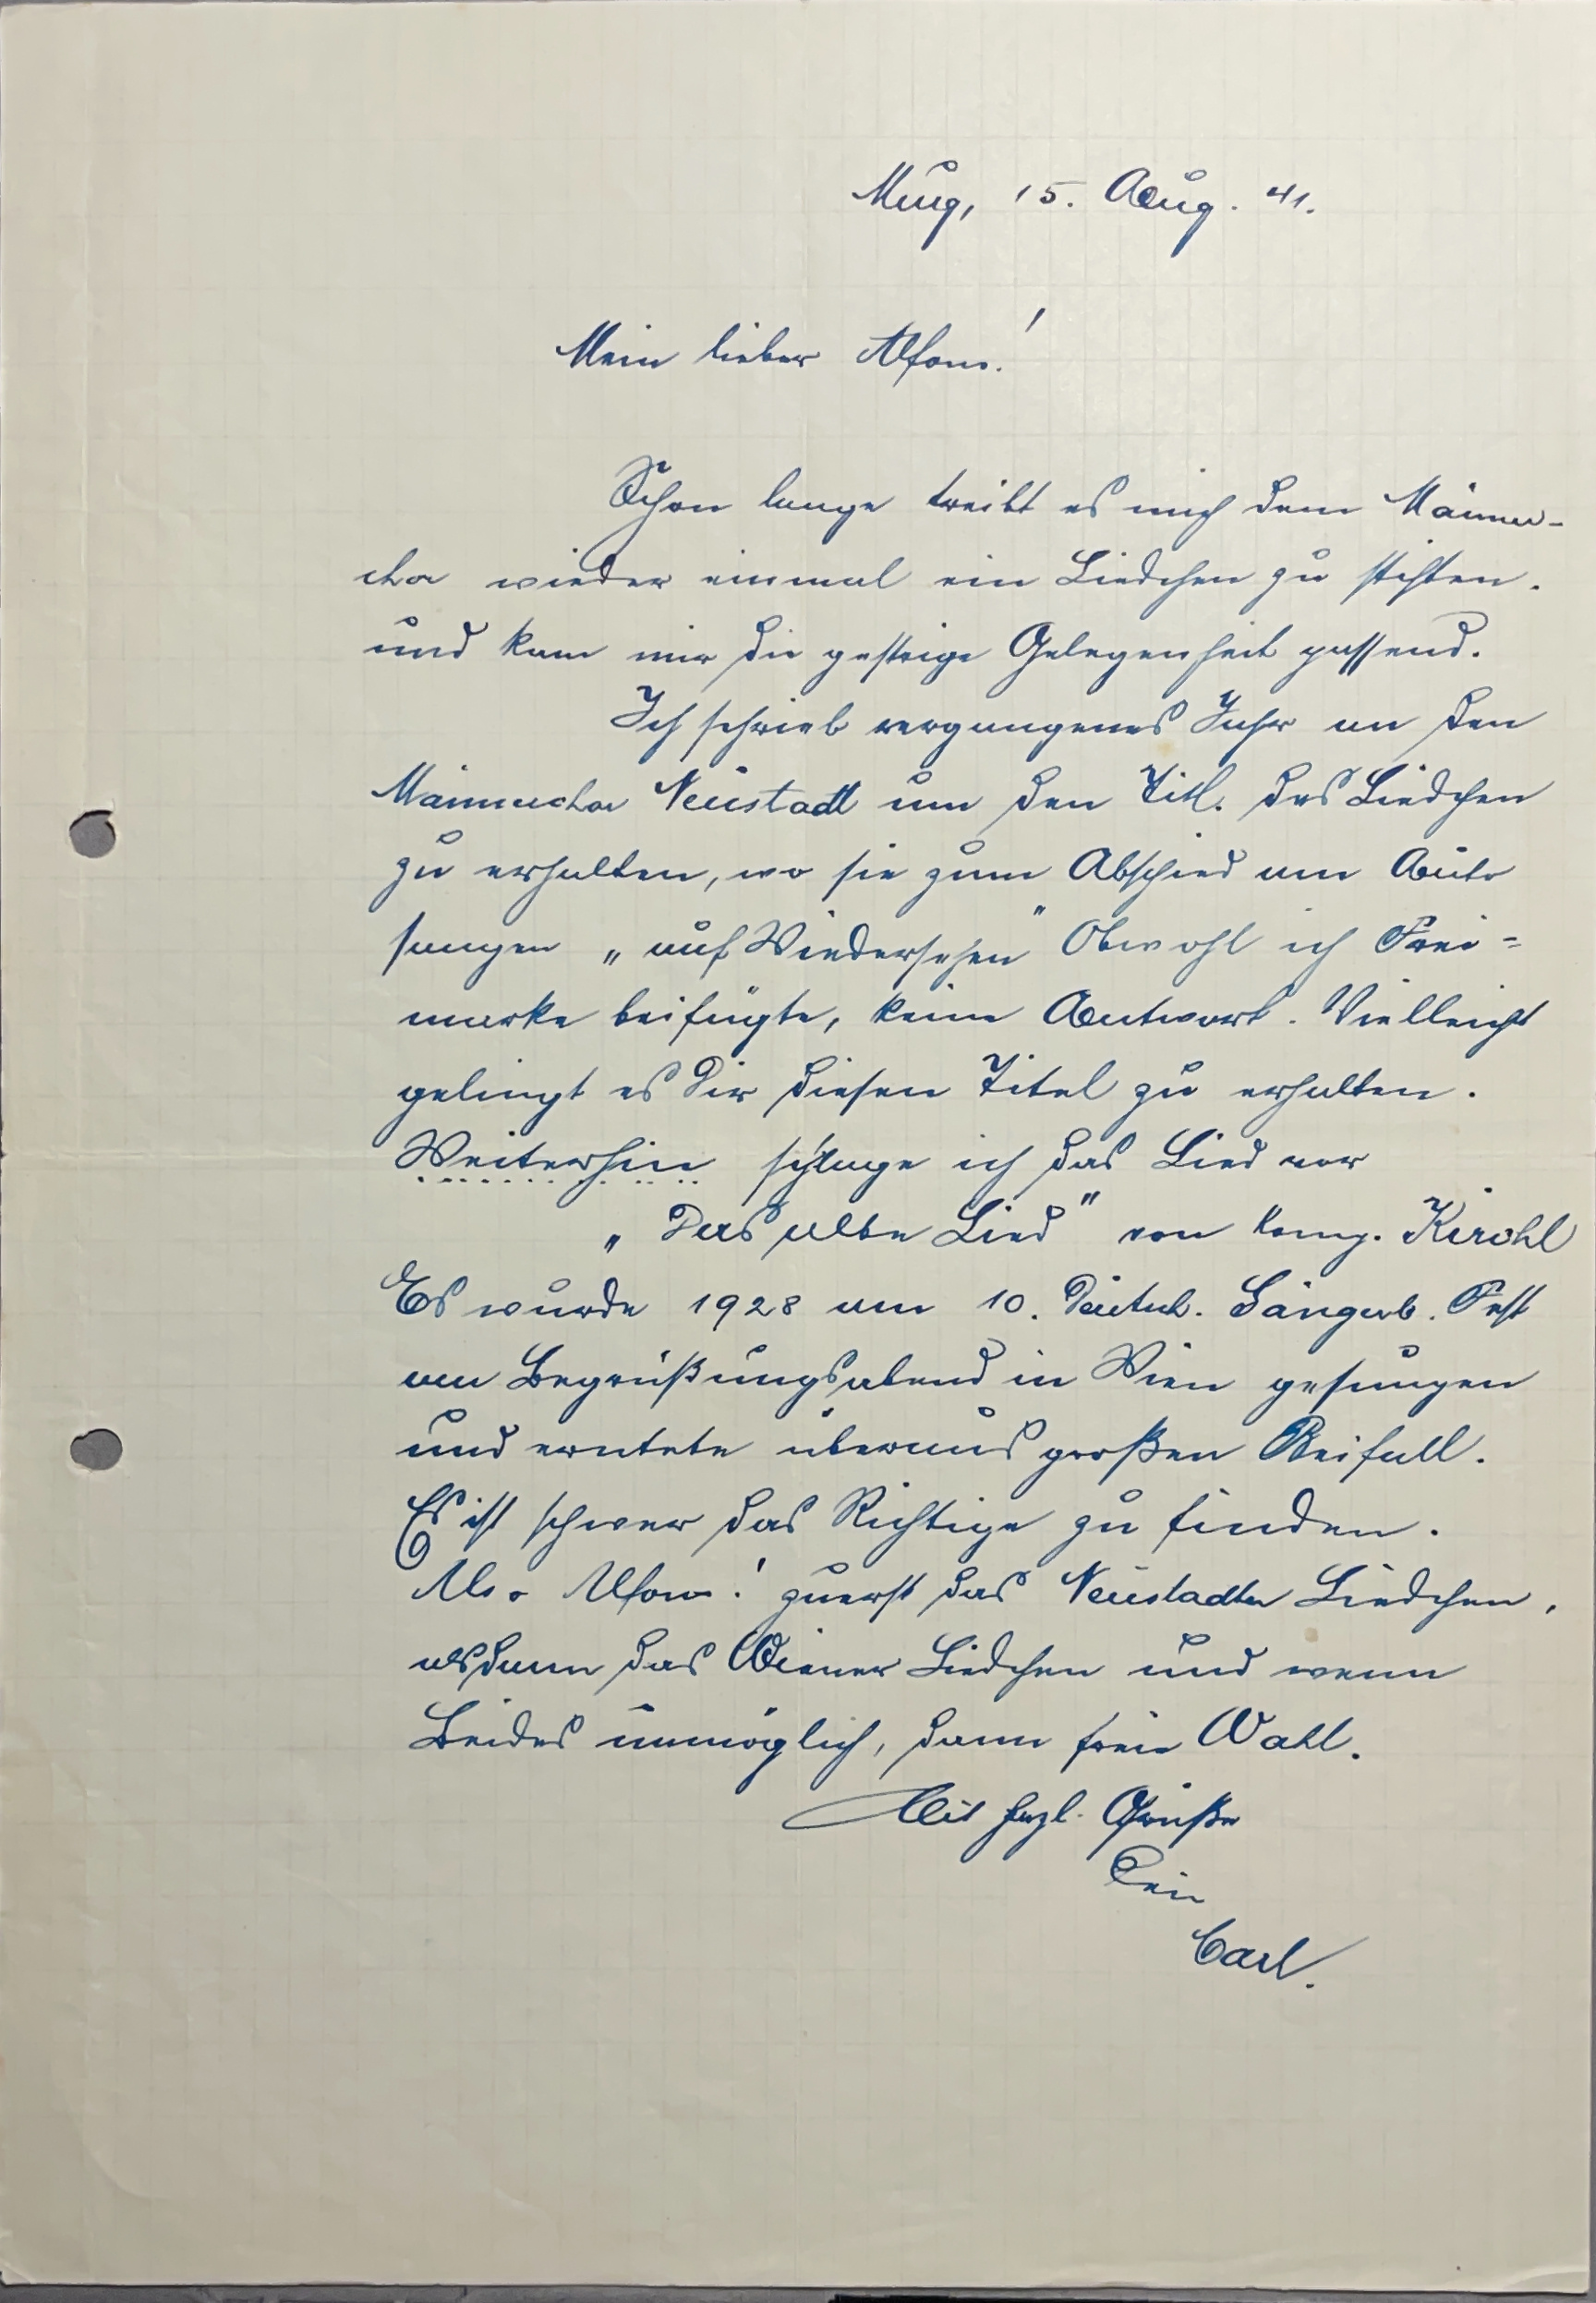
\includegraphics[width=\textwidth]{./assets/Images/Akte_076_S001.jpg}
      \caption{Beispiel für handschriftlichen Text in Akte\_076 erkannt mit Transkribus}
      \label{fig:transkribus-handschrift}
    \end{figure}

  \begin{figure}[htbp]
  \centering
  \begin{tcolorbox}[colback=oldLetter, colframe=black, sharp corners, width=\textwidth]
    Murg. 15. Aug 41 \\
    \\
    Mein lieber Alfons! \\
    Sehen lunge Lreitt es mich dem Männer- \\
    chor wieder einmal ein Liedehen zu stehten. \\
    und kam mir die gestege Gelegenheit gussend. \\
    Männechor Venstad um den Title das Liedchen \\
    zu erhalten, wo sie zum Abschied am Aute \\
    sängen „auf Wiederschen Owohl ich Frei! \\
    märke beifügte, keine Aentwarb. Vielleicht \\
    gelingt es Dir diesen Iitel zu erhalten. \\
    Weiterhin sänge ich fal Lied nur \\
    "Bas alte Lied von being. Rerohl \\
    Es wurde 1928 am 10. Dachub. Sängerb. Frst \\
    von Begrüßungsabend in Dien gesungen. \\
    und erntete überaus großen Reifall. \\
    Es ich schwer das Richtige zu finden. \\
    Aler Alfon, werst das Vemsladler Liedchen. \\
    alsdann das Biener Lidchen und wenn \\
    Leides unmöglich, dann freu Nall. \\
    Mit herzl. Grüße \\
    Dein \\
    Carl \\
  \end{tcolorbox}
  \caption{Transkription von \autoref{fig:transkribus-handschrift}}
  \label{fig:transkription-brief}
\end{figure}

    ChatGPT produziert daraus:

  \begin{figure}[htbp]
  \centering
    \begin{tcolorbox}[colback=oldLetter, colframe=black, sharp corners, width=\textwidth]
    Murg, 15. Aug. 41\\
    \\
Mein lieber Alfons!\\
\\
Schon lange treibt es mich, dem Männerchor wieder einmal ein Liedchen zu stiften, und kam mir die günstige Gelegenheit gelegen.\\
Ich schrieb vergangenes Jahr an den Männerchor Venstad, um den Titel des Liedchens zu erhalten, das sie zum Abschied am Auto sangen: „Auf Wiedersehen, o wohl ich frei!“\\
Ich fügte eine Frankierung bei, erhielt jedoch keine Antwort. Vielleicht gelingt es Dir, diesen Titel zu erhalten.\\
\\
Weiterhin sang ich das Lied nur „Das alte Lied von Wien“. Obwohl es am 10. Dezember 1928 beim Sängerbund-Fest von Begrüßungsabend in Wien gesungen wurde und überaus großen Beifall erntete, ist es schwer, das Richtige zu finden.\\

Aber Alfons, zuerst das Venstadler Liedchen, dann das Wiener Liedchen und wenn beides unmöglich, dann Fröhlichsein.\\

Mit herzlichen Grüßen\\
Dein\\
Carl\\
\end{tcolorbox}
\caption{Transkription durch ChatGPT von \autoref{fig:transkription-brief}}
  \label{fig:brief-carl-alfons}
\end{figure}

Durch CHatGPT verliert der Text zwar seine ursprüngliche Formatierung und Zeilenumbrüche, aber wird nun nahezu fehlerfrei lesbar. Nur das "Venstadler Liedchen" ist eigendlich eines aus "Neustadt". Eine anschliessende menschliche Korrektur ermöglicht also den Abgeleich mit dem nun lesbaren Text, und die Korrektur der Transkribtion.

Korrigiert und getagt lautet der Brief nun:
  \begin{figure}[htbp]
  \centering
\begin{tcolorbox}[colback=oldLetter, colframe=black, sharp corners, width=\textwidth]
  \textbf{\colorbox{place}{\texttt{Murg}}}.  \textbf{\colorbox{date}{\texttt{15. Aug 41}}} \\
\\
Mein lieber  \textbf{\colorbox{person}{\texttt{Alfons}}}!\\
Seit langem treibt es mich dem  \textbf{\colorbox{organization}{\texttt{Männer-}}}\\
\textbf{\colorbox{organization}{\texttt{chor}}} wieder einmal ein Liedchen zu stiften.\\
und kam mir die günstige Gelegenheit passend.\\
Ich schrieb vergangenes Jahr an den\\
Männechor Vorstand um den Titel das Liedchen\\
zu erhalten, wo sie zum Abschied am Auto \\
sangen "auf Wiederschen" Obwohl ich  \textbf{\colorbox{unclear}{\texttt{Frank-}}}\\
marke beifügte, keine Antwort. Vielleicht\\
gelingt es Dir diesen Titel zu erhalten.\\
Weiterhin sänge ich das Lied nur\\
"Das alte Lied" von  \textbf{\colorbox{abbrev}{\texttt{Komp.}}}\textbf{\colorbox{person}{\texttt{ Kirchl}}}\\
Es wurde \textbf{\colorbox{date}{\texttt{1928}}} am \textbf{\colorbox{eventTag}{\texttt{10. Deutsch. Sängerb. Fest}}}\\
am Begrüßungsabend in \textbf{\colorbox{place}{\texttt{Wien}}} gesungen.\\
und erntete überaus großen Beifall.\\
Es ich schwer das Richtige zu finden.\\
Also \textbf{\colorbox{person}{\texttt{Alfons}}}! zuerst das \textbf{\colorbox{place}{\texttt{Neustadter}}} Liedchen.\\
alsdann das \textbf{\colorbox{place}{\texttt{Wiener}}} Liedchen und wenn\\
Beides unmöglich, dann freie Wahl.\\
Mit herzl. Grüßen \\
Dein\\
\textbf{\colorbox{person}{\texttt{Carl}}}\\
\end{tcolorbox}
\caption{Tagging von \autoref{fig:brief-carl-alfons}}
  \label{fig:Tagging-brief-carl-alfons}
\end{figure}


\begin{tcolorbox}[colback=oldLetter, colframe=black, sharp corners, width=\textwidth]
\textbf{\colorbox{place}{\texttt{München}}}, \textbf{\colorbox{date}{\texttt{28.V.1941}}} \\
\\
Lieber \textbf{\colorbox{person}{\texttt{Otto}}}!\\
Nur wer die Sehnsucht kennt weiß was ich leide\\
Ich wandle traurig her in schwarzer Seide.\\
Die Sehnsucht brennt, du bist so fern.\\
Ach lieber \textbf{\colorbox{person}{\texttt{Otto}}}, wie hab ich dich gern.\\
Ich schnitt es gern in alle Rinden.\\
Ach \textbf{\colorbox{person}{\texttt{Otto}}}, wann u. wo kann ich dich finden?\\
Deine dich nie vergessende\\
\textbf{\colorbox{person}{\texttt{Lina Fingerdick}}}\\
\\
An\\
\textbf{\colorbox{person}{\texttt{Herrn Otto Bollinger}}}\\
z.Hd. \textbf{\colorbox{person}{\texttt{Herrn Alfons Zimmermann}}}\\
\textbf{\colorbox{organization}{\texttt{Vereinsführer des Männerchor}}}\\
\textbf{\colorbox{place}{\texttt{Murg}}}\\
\textbf{\colorbox{place}{\texttt{Laufenburg (Baden)}}}\\
\textbf{\colorbox{place}{\texttt{Rhina}}}
\end{tcolorbox}




\subsection{Diagram english}

\vspace{6\baselineskip}


\begin{center}
\resizebox{0.9\textwidth}{!}{
\begin{tikzpicture}[
  module/.style={rectangle, draw=black, fill=blue!10, thick, minimum width=4.5cm, minimum height=1.2cm, align=center},
  process/.style={rectangle, draw=black, fill=orange!20, thick, minimum width=4.8cm, minimum height=1.2cm, align=center},
  source/.style={rectangle, draw=black, fill=green!30!gray!20, thick, minimum width=4.2cm, minimum height=0.7cm, align=center},
  group/.style={draw=gray, dashed, rounded corners, inner sep=0.5cm},
  arrow/.style={-Latex, thick}, arrowboth/.style={<Latex>-<Latex>, thick},
  node distance=0.8cm and 1.6cm
]


% --- Hauptquellen oben ---
\node[source] (transkribus) at (-14.5, 0) {\textbf{app.transkribus.org} \\ Transcription};
\node[process] (dir) at (0, -3.2) {\textbf{File Directory} \\ with XML-Files};
\node[process] (llmpre) at (6, -3.2) {\textbf{llm\_XML\_preprocessing.py}};
\node[process, below=7.5cm of dir] (main) {\textbf{Transkribus\_II\_Test.py} \\ Main Processing};

% ------------------- MODULE (FLOWCHART) ------------------------
\node[module, below=2cm of main] (init) {Initialization \\ (CSV import, matcher)};
\node[module, below=of init]    (xml)  {XML \& Custom Tags \\ Parse, extract\_metadata};


% Referenzpunkt zentriert unter xml
\coordinate (modcenter) at ($(xml.south) + (0,-1.8)$);
\node[module] (roles)   at ($(modcenter) + (-8cm, -0.5)$) {Roles \\ assign, enrich};
\node[module] (persons) at ($(modcenter) + (-2.7cm, -0.5)$) {Persons \\ match, split, enrich};
\node[module] (orgs)    at ($(modcenter) + (2.7cm, -0.5)$)  {Organizations \\ extract, deduplicate};
\node[module] (places)  at ($(modcenter) + (8cm, -0.5)$)  {Places \\ context + combination};
\node[module] (dates)   at ($(modcenter) + (13cm, -0.5)$) {Dates \\ combine\_dates(), count};
\node[module] (events)  at ($(modcenter) + (-13.5cm, -0.5)$)  {Events \\ extract\_events\_from\_xml()};
\node[module, below=1.2cm of persons] (authors) {Authors \& Recipients \\ infer, deduplicate, score};
\node[module] (json)  at ($(modcenter) + (0cm, -7.5cm)$)  {BaseDocument Build \\ + Role Postprocessing};
\node[coordinate] (joinpoint) at ($(json.north) + (0, 1.5cm)$) {};
\node[coordinate] (joinpointxml) at ($(xml.south) + (0, -0.5cm)$) {};
\node[module, below=of json] (save) {Saving \\ JSON per page + total\_json};

% CSV-Quellen
\node[source] (csv1) at ($(transkribus.south) + (0.5, -4.5)$) {\textbf{export-person.csv}};
\node[source, below=0.6cm of csv1] (csv2) {\textbf{export-place.csv}};
\node[source, below=0.6cm of csv2] (csv3) {\textbf{export-roles.csv}};
\node[source, below=0.6cm of csv3] (csv4) {\textbf{export-organisationen.csv}};

\node[group, fit=(csv1)(csv2)(csv3)(csv4), name=nodegoatbox,
  label={[anchor=north west, xshift=-0.5cm, yshift=0.7cm]north west:\texttt{preprocessing: Nodegoat-export}}] {};

\node[group, fit=(transkribus), name=pretranskribusbox,
  label={[anchor=north west, xshift=-0.5cm, yshift=0.7cm]north west:\texttt{preprocessing: Transkribus}}] {};

  % --- Gruppenrahmen für Modulblock ---
\node[group, fit=
  (persons)(authors)(roles)
  (orgs)(dates)(events)
  (places)(joinpoint), name=flowchartbox] {};

% --- Gruppenrahmen um Hauptverarbeitung + Flowchart ---
\node[group, fit=(main)(flowchartbox)(save),
  label={[anchor=north west, xshift=12.5cm, yshift=+0.7cm]north west:\texttt{ Main Processing of the Pipeline}}] {};


% Verbindungen
\draw[arrow] (transkribus.east) -- ++(1.2,0)-- ++(0,-3.2)-- node[pos=0.6, left, font=\small, xshift=-2cm, yshift=1.3cm]{\textit{Export as XML}} (dir.west);  
\draw[arrow] (dir.east) -- (llmpre.west);
\draw[arrow] (llmpre.north) -- ++(0,1.2) -| node[pos=0.5, above, font=\small, xshift=3cm] {\textit{Custom-Tags}} (dir.north);
\draw[arrow] (dir.south) -- (main.north);
\draw[arrow] (main.south) -- (init.north);
\draw[arrow] (init.south) -- (xml.north);

\draw[arrow] (xml.south) -- (joinpointxml.south);
\draw[arrow] (joinpointxml) -- ($(roles.north |- joinpointxml)$) -- (roles.north);
\draw[arrow] (joinpointxml) -- ($(persons.north |- joinpointxml)$) -- (persons.north);
\draw[arrow] (joinpointxml) -- ($(orgs.north |- joinpointxml)$) -- (orgs.north);
\draw[arrow] (joinpointxml) -- ($(places.north |- joinpointxml)$) -- (places.north);
\draw[arrow] (joinpointxml) -- ($(dates.north |- joinpointxml)$) -- (dates.north);
\draw[arrow] (joinpointxml) -- ($(events.north |- joinpointxml)$) -- (events.north);

\draw[arrow, dashed] (persons.south) -- (authors.north);
\draw[arrow] (persons.west) -- (roles.east);
\draw[arrow] (roles.east) -- (persons.west);   
\draw[arrow] (persons.east) -- (orgs.west);
\draw[arrow] (orgs.west) -- (persons.east); 
\draw[arrow] (persons.east) -- (orgs.west);
\draw[arrow] (orgs.west)-- (persons.east)  ;      
\draw[arrow] (orgs.east) -- (places.west);  
\draw[arrow] (places.west) -- (orgs.east);   
             
% Doppelte Pfeile mit definiertem Stil
\draw[arrow] (events.south) -- ($(events.south |- joinpoint)$);
\draw[arrow] ($(events.south |- joinpoint)$) -- (joinpoint);

\draw[arrow] (roles.south) -- ($(roles.south |- joinpoint)$);
\draw[arrow] ($(roles.south |- joinpoint)$) -- (joinpoint);

\draw[arrow] (authors.south) -- ($(authors.south |- joinpoint)$);
\draw[arrow] ($(authors.south |- joinpoint)$) -- (joinpoint);

\draw[arrow] (orgs.south) -- ($(orgs.south |- joinpoint)$);
\draw[arrow] ($(orgs.south |- joinpoint)$) -- (joinpoint);

\draw[arrow] (places.south) -- ($(places.south |- joinpoint)$);
\draw[arrow] ($(places.south |- joinpoint)$) -- (joinpoint);

\draw[arrow] (dates.south) -- ($(dates.south |- joinpoint)$);
\draw[arrow] ($(dates.south |- joinpoint)$) -- (joinpoint);

\draw[arrow] (joinpoint.south) -- (json.north);
\draw[arrow] (json.south) -- (save.north);
\draw[arrow] 
  (nodegoatbox.south) |- ([xshift=-0.4cm]init.west)
  node[pos=0.6, left, font=\small, xshift=2.6cm, yshift=2.8cm]{\textit{delivers Groundtruth}};
\end{tikzpicture}
}
\end{center}
\vspace{6\baselineskip}


\vspace{6\baselineskip}


\begin{center}
\begin{tikzpicture}

% TikZ styles
\tikzset{
  module/.style={rectangle, draw=black, fill=blue!10, minimum width=0.4cm, minimum height=0.2cm},
  highlight/.style={rectangle, draw=black, fill=blue!40, minimum width=0.4cm, minimum height=0.2cm},
  arrow/.style={-stealth, line width=0.15mm},
  arrowboth/.style={stealth-stealth, line width=0.15mm},
  process/.style={rectangle, draw=black, fill=orange!20, thick, minimum width=6cm, minimum height=1cm, align=center},
  large/.style={rectangle, draw=black, fill=blue!10, thick, minimum width=4.5cm, minimum height=1.2cm, align=center}
}
%==========================
% Mini-Diagramm oben rechts
%==========================

\begin{scope}[shift={(9,0)}]
\node at (0, -3.7) {\textit{Above: Overall schema overview}};
\node[module] (init) at (0,0) {};
\node[module] (xml) at (0, -0.5) {};
\node[module]    (events)  at (-2.0, -1.3) {};
\node[module]    (roles)   at (-1.2, -1.3) {};
\node[highlight] (persons) at (-0.4, -1.3) {};
\node[module]    (orgs)    at ( 0.4, -1.3) {};
\node[module]    (places)  at ( 1.2, -1.3) {};
\node[module]    (dates)   at ( 2.0, -1.3) {};
\node[module] (authors)    at (-0.4, -2  ) {};
\node[module] (json)       at (-0,  -2.8 ) {};
\node[module] (save)       at (-0, -3.3  ) {};
\node[coordinate] (joinpoint) at ($(xml.south) + (0, -1.8cm)$) {};
\node[coordinate] (joinpointxml) at ($(xml.south) + (0, -0.3cm)$) {};

\draw[arrow, dashed] (persons.south) -- (authors.north);
\draw[arrow] (joinpoint.south) -- (json.north);
\draw[arrow] (json.south) -- (save.north);
\draw[arrow] (init.south) -- (xml.north);
\draw[arrowboth] (roles.east) -- (persons.west);
\draw[arrowboth] (persons.east) -- (orgs.west);
\draw[arrowboth] (orgs.east) -- (places.west);
%Pfeile oben
\draw[arrow] (xml.south) -- (joinpointxml.south);
\draw[arrow] (joinpointxml) -- ($(roles.north |- joinpointxml)$) -- (roles.north);
\draw[arrow] (joinpointxml) -- ($(persons.north |- joinpointxml)$) -- (persons.north);
\draw[arrow] (joinpointxml) -- ($(orgs.north |- joinpointxml)$) -- (orgs.north);
\draw[arrow] (joinpointxml) -- ($(places.north |- joinpointxml)$) -- (places.north);
\draw[arrow] (joinpointxml) -- ($(dates.north |- joinpointxml)$) -- (dates.north);
\draw[arrow] (joinpointxml) -- ($(events.north |- joinpointxml)$) -- (events.north);

%Pfeile unten
 Doppelte Pfeile mit definiertem Stil
\draw[arrow] (events.south) -- ($(events.south |- joinpoint)$);
\draw[arrow] ($(events.south |- joinpoint)$) -- (joinpoint);

\draw[arrow] (roles.south) -- ($(roles.south |- joinpoint)$);
\draw[arrow] ($(roles.south |- joinpoint)$) -- (joinpoint);

\draw[arrow] (authors.south) -- ($(authors.south |- joinpoint)$);
\draw[arrow] ($(authors.south |- joinpoint)$) -- (joinpoint);

\draw[arrow] (orgs.south) -- ($(orgs.south |- joinpoint)$);
\draw[arrow] ($(orgs.south |- joinpoint)$) -- (joinpoint);

\draw[arrow] (places.south) -- ($(places.south |- joinpoint)$);
\draw[arrow] ($(places.south |- joinpoint)$) -- (joinpoint);

\draw[arrow] (dates.south) -- ($(dates.south |- joinpoint)$);
\draw[arrow] ($(dates.south |- joinpoint)$) -- (joinpoint);

\draw[arrow] (joinpoint.south) -- (json.north);
\draw[arrow] (json.south) -- (save.north);
\end{scope}

% Large process diagram
\node[large] (personsmod) at (0,0) {\textbf{Persons} \\ match, split, enrich};

\node[process, below=1.2cm of personsmod] (split)  {\textbf{def split\_and\_enrich\_persons} \\ \textit{(Extract raw persons from XML or LLM)}};

\node[process, below=of split] (parse)  {\textbf{def extract\_person\_data} \\ (Split names, detect titles \& role expressions)};

\node[process, below=of parse] (match)  {\textbf{def match\_person} \\ (Fuzzy/contextual matching with groundtruth)};

\node[process, below=of match] (roles)  {\textbf{def assign\_roles\_to\_known\_persons} \\ (Assign roles \& organizations from modules)};

\node[large, right=2.8cm of roles] (rolematch) {\textbf{Role-Matcher.py} \\ (Provides normalized \\ roles)};

\node[large, above=1.3cm of rolematch] (orgmatch) {\textbf{Organization-Matcher.py} \\ (Provides normalized \\ organizations)};

\node[process, below=of roles] (score)  {\textbf{def calculate recipient\_score} \\ (Scoring based on transcript context)};

\node[process, below=of score] (dedup)  {\textbf{def deduplicate\_and\_group\_persons} \\ (Merge persons with same ID/name)};

\node[process, below=of dedup] (count)  {\textbf{def count\_mentions\_in\_transcript\_contextual} \\ (Count mentions in context, avoid duplicates)};

\node[below=of count, align=center] 
  {\textit{Top: process in person\_matcher.py}\\\textit{Right: input from role\_matcher.py and organization\_matcher.py}};

\draw[arrow] (personsmod.south) -- (split.north);
\draw[arrow] (split.south) -- (parse.north);
\draw[arrow] (parse.south) -- (match.north);
\draw[arrow] (match.south) -- (roles.north);
\draw[arrow] (roles.south) -- (score.north);
\draw[arrow] (score.south) -- (dedup.north);
\draw[arrow] (dedup.south) -- (count.north);

\draw[arrow] 
  (orgmatch.west) 
  -- ++(-0.5,0) 
  |- (roles.east);

\draw[arrow] (rolematch.west) -- (roles.east);

\node[draw=gray, dashed, rounded corners, inner sep=0.5cm, fit=(split)(count)] (group) {};
\end{tikzpicture}
\end{center}
\vspace{6\baselineskip}












        \subsubsection{Gründe für den Wechsel zu Nodegoat}
        \subsubsection{Nodegoat Modelierung}


  \subsection{Netzwerkanalyse als Methode}
        \subsubsection{Theoretischer Hintergrund der Netzwerkanalyse}
        \subsubsection{Ziele der Netzwerkanalyse im Kontext der Quellen}
        \subsubsection{Technische Umsetzung (Tools, Datenbankstruktur)}

\subsection{Normalisierung der Dateien --- von PDF zu JPEG}
\begin{minted}[
frame=lines,
framesep=2mm,
baselinestretch=1.2,
bgcolor=LightGray,
fontsize=\footnotesize,
linenos,
breaklines=true,   % Automatischer Zeilenumbruch
breakanywhere=true % Minted darf überall umbrechen (optional)
]{python}
import os
import fitz  # PyMuPDF

def convert_pdf_to_jpg(src_folder, dest_folder):
    # Überprüfen, ob der Zielordner existiert, und ihn ggf. erstellen
    if not os.path.exists(dest_folder):
        os.makedirs(dest_folder)

    # Durchgehen durch alle Dateien im Quellordner
    for root, dirs, files in os.walk(src_folder):
        for file in files:
            # Überprüfen, ob die Datei eine PDF-Datei ist
            if file.lower().endswith(".pdf"):
                # Vollständigen Pfad zur PDF-Datei erstellen
                pdf_path = os.path.join(root, file)
                # PDF-Datei öffnen
                doc = fitz.open(pdf_path)
                # Durch alle Seiten der PDF-Datei gehen
                for page_num in range(len(doc)):
                    page = doc[page_num]
                    # Seite in ein PixMap-Objekt umwandeln (für die Konvertierung in JPG)
                    pix = page.get_pixmap()
                    # Dateinamen ohne Dateiendung extrahieren
                    filename_without_extension = os.path.splitext(file)[0]
                    # Ausgabedateinamen erstellen mit führenden Nullen für die 
                    # Seitennummer
                    output_filename = f"{filename_without_extension}_S{page_num + 1:03d}.jpg"


                    # Vollständigen Pfad zur Ausgabedatei erstellen
                    output_path = os.path.join(dest_folder, output_filename)
                    # Bild speichern
                    pix.save(output_path)
                # PDF-Datei schließen
                doc.close()
                
                # Erfolgsmeldung ausgeben
                print(f"{file} wurde erfolgreich umgewandelt und gespeichert
                in {dest_folder}")

# Pfade zu den Ordnern mit den PDF-Dateien (Quelle) und den JPG-Dateien (Ziel)
src_folder = r"/Users/svenburkhardt/Documents/D_Murger_Männer_Chor_Forschung/Scan_Männerchor/Männerchor_Akten_1925–1945/Scan_Männerchor_PDF"
dest_folder = r"/Users/svenburkhardt/Documents/D_Murger_Männer_Chor_Forschung/Masterarbeit/JPEG_Akten_Scans"


# Funktion aufrufen, um die Konvertierung durchzuführen
convert_pdf_to_jpg(src_folder, dest_folder)

\end{minted}
\newpage
%--------------------------------------------------------------------------------------%
%--------------------------------------------------------------------------------------%
%------------------------          Aufbau der Datenbank        ----------------------------%
%--------------------------------------------------------------------------------------%
%--------------------------------------------------------------------------------------%

     \section{Aufbau der Datenbank}
    \subsection{Konzeption der Datenmodelieung}
      \subsubsection{Eigene Ontologie im Vergleich zu bestehenden Standards}
      \subsubsection{Verknüpfung von Personen, Orten und Ereignissen}
    
    \subsection{Implementierung der Datenbank}
      \subsubsection{Datenbankdesign}
      \subsubsection{Herausforderungen bei der Datenaufnahme}
      \subsubsection{Verknüpfung mit externen Quellen (z.B. Wikidata)}

    \newpage
%--------------------------------------------------------------------------------------%
%--------------------------------------------------------------------------------------%
%------------------------          Analyse der Netzwerke         ----------------------------%
%--------------------------------------------------------------------------------------%
%--------------------------------------------------------------------------------------%
\section{Analyse der Netzwerke}
  \subsection{Soziale Netzwerke des Vereinslebens}
    \subsubsection{Verbindungen zwischen Mitgliedern}
    \subsubsection{ Kooperationen mit anderen Vereinen}
\subsection{ Politische Netzwerke und deren Veränderungen}
    \subsubsection{Einfluss der NS-Diktatur auf die Netzwerke}
    \subsubsection{Feldpostkarten als Quelle für militärische Netzwerke}
    
 \subsection{ Geografische Ausdehnung der Netzwerke}
  \subsubsection{Einsatzorte der Chormitglieder während des Krieges}
  \subsubsection{ Lokale und überregionale Verbindungen}
  \newpage
%--------------------------------------------------------------------------------------%
%--------------------------------------------------------------------------------------%
%------------------------          Diskussion der Erebnisse         ----------------------------%
%--------------------------------------------------------------------------------------%
%--------------------------------------------------------------------------------------%
\section{Diskussion der Ergebnisse}
  \subsection{Sichtbarmachung der Netzwerke durch Nodegoat und Netzwerkanalyse}
  \subsection{Gibt es Veränderungen der Netzwerke im historischen Kontext?}
  \newpage

%--------------------------------------------------------------------------------------%
%--------------------------------------------------------------------------------------%
%------------------------           Bibliographie      --------------------------------%
%--------------------------------------------------------------------------------------%
%--------------------------------------------------------------------------------------%
\section{Bibliographie}

Referenzen, die noch nachzuschauen sind:

-- Akten\_Gesamtübersicht.csv im Anhang
\printbibliography[
heading=bibintoc,
title={References} % title of the 'references' section, change this if necessary
]

\end{document}
